\documentclass[svgnames,11pt]{beamer}
\input{/home/tof/Documents/Cozy/latex-include/preambule_commun.tex}
\input{/home/tof/Documents/Cozy/latex-include/preambule_beamer.tex}
%\usepackage{pgfpages} \setbeameroption{show notes on second screen=left}
\author[]{Christophe Viroulaud}
\title{Exercices constructions élémentaires\\ Éléments de correction}
\date{\framebox{\textbf{Lang 02}}}
%\logo{}
\institute{Première - NSI}

\begin{document}
\begin{frame}
\titlepage
\end{frame}
\section{Exercice 1}
\begin{frame}[fragile]
    \frametitle{Exercice 1}
    \begin{lstlisting}[language=Python , basicstyle=\ttfamily\small, xleftmargin=2em, xrightmargin=2em]
a = 3
\end{lstlisting}
    \begin{center}
        \begin{tikzpicture}
            \draw (0,1) -- (0,0) -- (1,0) -- (1,1);
            \node (3) at (-2,2) {3};
            \node at (.5,-.2) {a};
            \draw[->,>=latex] (3) to[bend left=40] (.5,.5);
            \draw (4,1) -- (4,0) -- (5,0) -- (5,1);
            \node at (4.5,.5) {3};
            \node at (4.5,-.2) {a};

        \end{tikzpicture}
        \captionof{figure}{Affectation}
    \end{center}

\end{frame}
\begin{frame}[fragile]
\begin{lstlisting}[language=Python , basicstyle=\ttfamily\small, xleftmargin=2em, xrightmargin=2em]
a = 4
\end{lstlisting}
    \begin{center}
        \begin{tikzpicture}
            \draw (0,1) -- (0,0) -- (1,0) -- (1,1);
            \node (3) at (.5,.5) {3};
            \node (4) at (-2,2) {4};
            \node at (.5,-.2) {a};
            \draw[->,>=latex] (4) to[bend left=40] (.5,.6);
            \draw (4,1) -- (4,0) -- (5,0) -- (5,1);
            \node at (4.5,.5) {4};
            \node at (4.5,-.2) {a};
        \end{tikzpicture}
        \captionof{figure}{Nouvelle affectation}
    \end{center}

\end{frame}
\begin{frame}[fragile]
    \begin{lstlisting}[language=Python , basicstyle=\ttfamily\small, xleftmargin=2em, xrightmargin=2em]
a = a + 2
\end{lstlisting}
    \begin{center}
        \begin{tikzpicture}
            \draw (0,1) -- (0,0) -- (1,0) -- (1,1);
            \node (3) at (.5,.5) {4};
            \node (4) at (.5,2) {4 + 2 = 6};

            \node at (.5,-.2) {a};
            \draw[->, dashed,>=latex] (3) to [bend left=60] (4.west);
            \draw (4,1) -- (4,0) -- (5,0) -- (5,1);
            \node at (4.5,.5) {6};
            \node at (4.5,-.2) {a};
            \draw[->, >=latex] (4.east) to [bend left=60](3.east);

        \end{tikzpicture}
        \captionof{figure}{Calcul puis affectation}
    \end{center}

\end{frame}
\begin{frame}[fragile]
    \begin{lstlisting}[language=Python , basicstyle=\ttfamily\small, xleftmargin=2em, xrightmargin=2em]
a = 2
\end{lstlisting}
    \begin{center}
        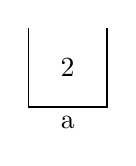
\begin{tikzpicture}
            \draw (0,1) -- (0,0) -- (1,0) -- (1,1);
            \node (3) at (.5,.5) {2};
            \node at (.5,-.2) {a};

        \end{tikzpicture}
    \end{center}

\end{frame}

\begin{frame}[fragile]
    \begin{lstlisting}[language=Python , basicstyle=\ttfamily\small, xleftmargin=2em, xrightmargin=2em]
b = a*a
\end{lstlisting}
    \begin{center}
        \begin{tikzpicture}
            \draw (0,1) -- (0,0) -- (1,0) -- (1,1);
            \node (3) at (.5,.5) {2};
            \node at (.5,-.2) {a};

            \draw (4,1) -- (4,0) -- (5,0) -- (5,1);
            \node (3) at (4.5,.5) {4};
            \node at (4.5,-.2) {b};

        \end{tikzpicture}
    \end{center}

\end{frame}
\begin{frame}[fragile]
    \begin{lstlisting}[language=Python , basicstyle=\ttfamily\small, xleftmargin=2em, xrightmargin=2em]
b = a*b
\end{lstlisting}
    \begin{center}
        \begin{tikzpicture}
            \draw (0,1) -- (0,0) -- (1,0) -- (1,1);
            \node (3) at (.5,.5) {2};
            \node at (.5,-.2) {a};

            \draw (4,1) -- (4,0) -- (5,0) -- (5,1);
            \node (3) at (4.5,.5) {8};
            \node at (4.5,-.2) {b};

        \end{tikzpicture}
    \end{center}

\end{frame}
\begin{frame}[fragile]
    \begin{lstlisting}[language=Python , basicstyle=\ttfamily\small, xleftmargin=2em, xrightmargin=2em]
b = b*b
\end{lstlisting}
    \begin{center}
        \begin{tikzpicture}
            \draw (0,1) -- (0,0) -- (1,0) -- (1,1);
            \node (3) at (.5,.5) {2};
            \node at (.5,-.2) {a};

            \draw (4,1) -- (4,0) -- (5,0) -- (5,1);
            \node (3) at (4.5,.5) {64};
            \node at (4.5,-.2) {b};

        \end{tikzpicture}
    \end{center}

\end{frame}
\begin{frame}[fragile]
    \frametitle{}

\begin{center}
\begin{lstlisting}[language=Python , basicstyle=\ttfamily\small, xleftmargin=2em, xrightmargin=2em]
print("i+") # affiche i+
print(i+) # message d'erreur: on essaie d'ajouter i à ... rien
\end{lstlisting}
\end{center}

\end{frame}
\begin{frame}[fragile]
    \begin{lstlisting}[language=Python , basicstyle=\ttfamily\small, xleftmargin=2em, xrightmargin=2em]
a = 2
\end{lstlisting}
    \begin{center}
        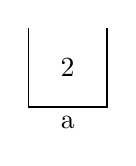
\begin{tikzpicture}
            \draw (0,1) -- (0,0) -- (1,0) -- (1,1);
            \node (3) at (.5,.5) {2};
            \node at (.5,-.2) {a};

        \end{tikzpicture}
    \end{center}

\end{frame}
\begin{frame}[fragile]
    \begin{lstlisting}[language=Python , basicstyle=\ttfamily\small, xleftmargin=2em, xrightmargin=2em]
b = 3
\end{lstlisting}
    \begin{center}
        \begin{tikzpicture}
            \draw (0,1) -- (0,0) -- (1,0) -- (1,1);
            \node (3) at (.5,.5) {2};
            \node at (.5,-.2) {a};

            \draw (4,1) -- (4,0) -- (5,0) -- (5,1);
            \node (3) at (4.5,.5) {3};
            \node at (4.5,-.2) {b};

        \end{tikzpicture}
    \end{center}

\end{frame}
\begin{frame}[fragile]
    \begin{lstlisting}[language=Python , basicstyle=\ttfamily\small, xleftmargin=2em, xrightmargin=2em]
tmp = a
\end{lstlisting}
    \begin{center}
        \begin{tikzpicture}
            \draw (0,1) -- (0,0) -- (1,0) -- (1,1);
            \node (3) at (.5,.5) {2};
            \node at (.5,-.2) {a};

            \draw (4,1) -- (4,0) -- (5,0) -- (5,1);
            \node (3) at (4.5,.5) {3};
            \node at (4.5,-.2) {b};

            \draw (8,1) -- (8,0) -- (9,0) -- (9,1);
            \node (3) at (8.5,.5) {2};
            \node at (8.5,-.2) {tmp};

        \end{tikzpicture}
    \end{center}

\end{frame}
\begin{frame}[fragile]
    \begin{lstlisting}[language=Python , basicstyle=\ttfamily\small, xleftmargin=2em, xrightmargin=2em]
a = b
\end{lstlisting}
    \begin{center}
        \begin{tikzpicture}
            \draw (0,1) -- (0,0) -- (1,0) -- (1,1);
            \node (3) at (.5,.5) {3};
            \node at (.5,-.2) {a};

            \draw (4,1) -- (4,0) -- (5,0) -- (5,1);
            \node (3) at (4.5,.5) {3};
            \node at (4.5,-.2) {b};

            \draw (8,1) -- (8,0) -- (9,0) -- (9,1);
            \node (3) at (8.5,.5) {2};
            \node at (8.5,-.2) {tmp};

        \end{tikzpicture}
    \end{center}

\end{frame}
\begin{frame}[fragile]
    \begin{lstlisting}[language=Python , basicstyle=\ttfamily\small, xleftmargin=2em, xrightmargin=2em]
b = tmp
\end{lstlisting}
    \begin{center}
        \begin{tikzpicture}
            \draw (0,1) -- (0,0) -- (1,0) -- (1,1);
            \node (3) at (.5,.5) {3};
            \node at (.5,-.2) {a};

            \draw (4,1) -- (4,0) -- (5,0) -- (5,1);
            \node (3) at (4.5,.5) {2};
            \node at (4.5,-.2) {b};

            \draw (8,1) -- (8,0) -- (9,0) -- (9,1);
            \node (3) at (8.5,.5) {2};
            \node at (8.5,-.2) {tmp};

        \end{tikzpicture}
    \end{center}
\begin{aretenir}[]
La séquence inverse (\emph{swap}) les valeurs de \textbf{\texttt{a}} et \textbf{\texttt{b}}.
\end{aretenir}
\begin{aretenir}[Remarque]
    Python facilite cette opération:
    \begin{lstlisting}[language=Python , basicstyle=\ttfamily\small, xleftmargin=2em, xrightmargin=2em]
a, b = b, a
\end{lstlisting}
    \end{aretenir}
\end{frame}
\section{Exercice 2}
\begin{frame}[fragile]
    \frametitle{Exercice 2}

\begin{center}
\begin{lstlisting}[language=Python , basicstyle=\ttfamily\small, xleftmargin=1em, xrightmargin=1em]
longueur = int(input("Longueur (en cm): "))
largeur = int(input("Largeur (en cm): "))
print("L'aire du rectangle est {}cm².".format(longueur*largeur))
\end{lstlisting}
\captionof{code}{Aire d'un rectangle}
\label{CODE}
\end{center}

\end{frame}
\section{Exercice 3}
\begin{frame}[fragile]
    \frametitle{Exercice 3}

\begin{center}
\begin{lstlisting}[language=Python , basicstyle=\ttfamily\small, xleftmargin=1em, xrightmargin=1em]
age = int(input("Quel est votre âge? "))
if age >= 18:
    print("Vous êtes majeur.")
else:
    print("Vous êtes mineur.")
\end{lstlisting}
\captionof{code}{Âge}
\label{CODE}
\end{center}
\begin{aretenir}[Remarque]
    \texttt{\textbf{input}} renvoie une chaîne de caractère (\texttt{\textbf{string}}).
    Il faut la convertir en entier (\texttt{\textbf{int}}).
\end{aretenir}
\end{frame}
\section{Exercice 4}
\begin{frame}[fragile]
    \frametitle{Exercice 4}

\begin{center}
\begin{lstlisting}[language=Python , basicstyle=\ttfamily\small, xleftmargin=1em, xrightmargin=1em]
age = int(input("Quel est votre âge? "))
if age < 16:
    print("Le prix de la carte est 10€.")
else:
    if age <= 25:
    ...
\end{lstlisting}
\captionof{code}{Cinéma - première version}
\label{CODE}
\end{center}   

\end{frame}
\begin{frame}[fragile]
    \frametitle{Exercice 4}

\begin{center}
\begin{lstlisting}[language=Python , basicstyle=\ttfamily\small, xleftmargin=1em, xrightmargin=1em]
age = int(input("Quel est votre âge? "))
if age < 16:
    print("Le prix de la carte est 10€.")
elif age <= 25:
    print("Le prix de la carte est 15€.")
elif age <= 59:
    print("Le prix de la carte est 25€.")
else:
    print("Le prix de la carte est 15€.")
\end{lstlisting}
\captionof{code}{Cinéma - seconde version}
\label{CODE}
\end{center}   
\begin{aretenir}[Remarque]
Ligne 4: inutile de vérifier si age >= 16, c'est
forcément le cas.
\end{aretenir}
\end{frame}
\section{Exercice 5}
\begin{frame}[fragile]
    \frametitle{Exercice 5}

\begin{center}
\begin{lstlisting}[language=Python , basicstyle=\ttfamily\small, xleftmargin=1em, xrightmargin=1em]
from random import randint

somme = 0
for i in range(10):
    nb = randint(1, 10)
    somme += nb
print(somme)
\end{lstlisting}
\captionof{code}{Somme}
\label{CODE}
\end{center}   
\begin{aretenir}[Remarque]
Ne pas oublier d'importer la bibliothèque.
\end{aretenir}
\end{frame}
\section{Exercice 6}
\begin{frame}[fragile]
    \frametitle{Exercice 6}

\begin{center}
\begin{lstlisting}[language=Python , basicstyle=\ttfamily\small, xleftmargin=1em, xrightmargin=1em]
from random import randint

nb = randint(1,10)
essai = 0
trouve = False
while not trouve:
    proposition = int(input("Quel nombre? "))
    if proposition == nb:
        trouve = True
    essai += 1
print(essai)
\end{lstlisting}
\captionof{code}{Deviner - première version}
\label{CODE}
\end{center}   
\begin{aretenir}[Remarque]
On utilise une variable \emph{booléenne}. 
\end{aretenir}
\end{frame}
\begin{frame}[fragile]
\begin{center}
\begin{lstlisting}[language=Python , basicstyle=\ttfamily\small, xleftmargin=1em, xrightmargin=1em]
from random import randint

nb = randint(1,10)
essai = 1
# compare la proposition de l'utilisateur à nb
while not(int(input("Quel nombre? ")) == nb):
    essai += 1
print(essai)
\end{lstlisting}
\captionof{code}{Deviner - première version}
\label{CODE}
\end{center}   
\begin{aretenir}[Remarque]
On compare directement l'entrée avec la valeur de \textbf{\texttt{nb}}.
\end{aretenir}
\end{frame}
\section{Exercice 7}
\begin{frame}
    \frametitle{Exercice 7}
    \begin{itemize}
        \item 20/3 renvoie le résultat de la division. Nous reviendrons plus tard sur le \emph{type} de ce résultat.
        \item 20//3 renvoie la partie entière de la division. C'est un \emph{entier}.
        \item 20\%3 renvoie le reste de la division. C'est un \emph{entier}. On appelle cette opération le \emph{modulo}.
        \end{itemize}
    

\end{frame}
\begin{frame}[fragile]
    \frametitle{}

\begin{center}
\begin{lstlisting}[language=Python , basicstyle=\ttfamily\small, xleftmargin=2em, xrightmargin=2em]
secondes = int(input("Donnez le nombre de secondes: "))
heures = secondes // 3600
minutes = (secondes % 3600) // 60
secondes = (secondes % 3600) % 60
\end{lstlisting}
\captionof{code}{Durée}
\label{CODE}
\end{center}

\end{frame}
\begin{frame}[fragile]
    \frametitle{}

\begin{center}
\begin{lstlisting}[language=Python , basicstyle=\ttfamily\small, xleftmargin=2em, xrightmargin=2em]
if heures < 10:
    heures = "0"+str(heures)
if minutes < 10:
    minutes = "0"+str(minutes)
if secondes < 10:
    secondes = "0"+str(secondes)
print("{}h {}min {}s".format(heures, minutes, secondes))
\end{lstlisting}
\captionof{code}{Affichage}
\label{CODE}
\end{center}
\begin{aretenir}[Remarque]
Les variables sont des entiers et deviennent des chaînes de caractères (string). Python permet de changer le type d'une variable. Ce n'est pas le cas de tous les langages.
\end{aretenir}
\end{frame}
\section{Exercice 8}
\begin{frame}[fragile]
    \frametitle{Exercice 8}

\begin{center}
\begin{lstlisting}[language=Python , basicstyle=\ttfamily\small, xleftmargin=1em, xrightmargin=1em]
nb = int(input("Quelle table? "))
for i in range(11): # 11 signifie qu'il il y aura 11 tours
    print(f"{i}×{nb} = {i*nb}")
\end{lstlisting}
\captionof{code}{Multiplication}
\label{CODE}
\end{center} 
\begin{aretenir}[Remarque]
    Noter ici le f en début de ligne qui est une autre manière de formater le texte (pour des versions
    récentes de Python (>=3.6)). Il est possible d'écrire:
\begin{lstlisting}[language=Python , basicstyle=\ttfamily\small, xleftmargin=2em, xrightmargin=2em]
print("{}×{} = {}".format(i,nb,i*nb))
\end{lstlisting}
\end{aretenir}
\end{frame}
\section{Exercice 9}
\begin{frame}[fragile]
    \frametitle{Exercice 9}

\begin{center}
\begin{lstlisting}[language=Python , basicstyle=\ttfamily\small, xleftmargin=2em, xrightmargin=2em]
for i in range(10,-1,-1):
    # range(premier terme (inclus), dernier terme (exclu), pas)
    print(i)
\end{lstlisting}
\captionof{code}{Compte à rebours}
\label{CODE}
\end{center}

\end{frame}
\section{Exercice 10}
\begin{frame}[fragile]
    \frametitle{Exercice 10}

\begin{center}
\begin{lstlisting}[language=Python , basicstyle=\ttfamily\small, xleftmargin=2em, xrightmargin=2em]
for i in range(2,25,2):
    print(i, end=" ")
\end{lstlisting}
\captionof{code}{Nombres pairs}
\label{CODE}
\end{center}
\begin{aretenir}[Remarque]
    L'option \texttt{\textbf{end}} de \texttt{\textbf{print}} définit le caractère à mettre en fin de ligne (retour chariot par défaut).
\end{aretenir}
\end{frame}
\section{Exercice 11}
\begin{frame}[fragile]
    \frametitle{Exercice 11}

\begin{center}
\begin{lstlisting}[language=Python , basicstyle=\ttfamily\small, xleftmargin=1em, xrightmargin=1em]
somme = 0
for i in range(10):
    somme += int(input("note: "))
\end{lstlisting}
\captionof{code}{Moyenne}
\label{CODE}
\end{center}
\begin{aretenir}[Remarque]
    Il faut noter ici l'ordre dans lequel l'interprète
    lit cette ligne:
\begin{itemize}
    \item il lit la valeur du \texttt{\textbf{input}},
    \item il la convertit en entier,
    \item il additionne cette valeur à somme.
\end{itemize}
\end{aretenir}
\end{frame}
\begin{frame}[fragile]
\begin{center}
\begin{lstlisting}[language=Python , basicstyle=\ttfamily\small, xleftmargin=1em, xrightmargin=1em]
somme = 0
for i in range(10):
    somme += int(input("note: "))
moyenne = round(somme/10, 2)
\end{lstlisting}
\captionof{code}{Moyenne}
\label{CODE}
\end{center}
\begin{aretenir}[Remarque]
    La fonction \texttt{\textbf{round}} permet d'arrondir
    ici à 2 chiffres après la virgule
\end{aretenir}
\end{frame}
\begin{frame}[fragile]
    \begin{center}
    \begin{lstlisting}[language=Python , basicstyle=\ttfamily\small, xleftmargin=1em, xrightmargin=1em]
if moyenne >= 15:
    print("{}/20, félicitations!".format(moyenne))
elif moyenne >= 10:
    # il est inutile ici de vérifier si moyenne < 15
    print("{}/20, bon travail!".format(moyenne))
else:
    print("{}/20, doit fournir des efforts!".format(moyenne))
\end{lstlisting}
    \captionof{code}{Affichage}
    \label{CODE}
    \end{center}
    
    \end{frame}
\section{Exercice 11}
\begin{frame}[fragile]
    \frametitle{Exercice 11}

\begin{center}
\begin{lstlisting}[language=Python , basicstyle=\ttfamily\small, xleftmargin=1em, xrightmargin=1em]
mini = 0
maxi = 100
trouve = False
coups = 0

print("Pensez à un nombre entre 1 et 100.")
\end{lstlisting}
\captionof{code}{Devinette}
\label{CODE}
\end{center}  

\end{frame}
\begin{frame}[fragile]
    \frametitle{Exercice 11}

\begin{center}
\begin{lstlisting}[language=Python , basicstyle=\ttfamily\small, xleftmargin=1em, xrightmargin=1em]
while not trouve:
    coups += 1
    # choix de la valeur (milieu de l'intervalle)
    proposition = (mini + maxi)//2
    print("Le nombre est-il {}?".format(proposition))
    reponse = input("Merci de répondre = + ou -: ")
    if reponse == "=":
        print("J'ai trouvé en {} coups!".format(coups))
        trouve = True
    elif reponse == "+": # réduction de l'intervalle
        mini = proposition
    else: # réduction de l'intervalle
        maxi = proposition
\end{lstlisting}
\captionof{code}{Devinette}
\label{CODE}
\end{center}  

\end{frame}
\end{document}